
\documentclass{article}  
\usepackage{graphicx}
\usepackage[utf8]{inputenc}
\usepackage[T1]{fontenc}
\usepackage{float}
\usepackage[italian]{babel}
\usepackage{listings}
\usepackage[usenames]{color}
\usepackage{natbib}
\usepackage{siunitx}
\usepackage[strict]{changepage}
\usepackage{physics}
\usepackage{wrapfig}
\usepackage[a4paper, top=2cm, bottom=2cm, right=2cm, left=2cm]{geometry}
\usepackage{array}
\usepackage{color}
\usepackage{colortbl}
\usepackage{amsmath}
\usepackage{amssymb}
\usepackage{multirow}
\usepackage{enumitem}
\usepackage{hyperref}
\usepackage{times}
\usepackage{booktabs}
\usepackage{subfig}
\usepackage{multirow}



\title{Effetto Zeeman}
\author{Docente: dott. Garfagnini, dott. Lunardon \\
	Gruppo 14}
\date{Anno accademico 2019/20}

\begin{document}
	
	
	
	\maketitle
	
	\begin{itemize}
		\item[$\circ$] Aidin Attar - 1170698 - aidin.attar@studenti.unipd.it
		\item[$\circ$] Ema Baci - 1171107 – ema.baci@studenti.unipd.it
		\item[$\circ$] Alessandro Bianchetti – 1162147 – alessandro.bianchetti@studenti.unipd.it
	\end{itemize}
	
	\vspace{3 cm}
	\begin{large}\textsc{\textbf{Scopo dell'esperienza}: studio dell'effetto Zeeman per atomo di Neon, stima del fattore di Landè} 
	\end{large}
	\vspace{8.5cm}
	
	\begin{figure}[H]
		\centering
		\section{Conclusioni}
\includegraphics[scale = 0.5 , angle=0]{unipd_logo.png}
	\end{figure}
	
	%\newpage \tableofcontents \newpage
	
	\twocolumn
	
	\subsection*{Descrizione dell'apparato} 
	
	L'apparato sperimentale si compone di una lampada al Neon, capace di emettere
	radiazione elettromagnetica associta principlamente a transizioni tra 3p e 2p.
	In particolare siamo interessati alla transizione da $\lambda = $585.3 nm.
	Tale lampada è inserita all'interno di una cavità magnetica, per cui ci si 
	aspetta la comparsa di righe di emissione: tuttavia, considerando la 
	polarizzazione delle righe, possiamo “sopprimere” la transizione centrale
	orientando il campo magnetico in modo longitudinale alla linea di 
	osservazione, in modo tale da vedere solo le due righe marginali. 
	
	Il raggio di luce emessa passa quindi per una lente condensante, necessaria 
	per concentrare quanto più possibile il fascio, che passa quindi per una 
	fenditura e successivamente attraverso un prisma, necessario per ruotare di 
	$90\deg$ la luce e dividerla nelle sue componenti principali. 
	
	A questo punto i raggi incidono sulla lamina di Lummer-Gehrcke, dispositivo
	interferenziale ad alta risoluzione, in modo quasi
	radente (faremo in seguito una stima dell'angolo di incidenza) e il fascio 
	emergente viene infine focalizzato sul dispositivo ottico di lettura (un CCD
	monodimensionale) attraverso la lente di camera.
	
	%La presa dati di questa esperienza è stata svolta interamente da remoto; in 
	%particolare la connessione al PC del laboratorio avviene tramite 
	%l'esportazione dello schermo via VNC Viewer.
	
	L'acquisizione dei dati è avvenutatramite l'interfaccia di controllo dell'
	apparato, che permette di controllare le diverse componenti appena citate.
	
	Per l'analisi dati sono stati utilizzati programmi scritti in c++, root ed Excel.
	
	%\begin{center}
	%\begin{figure}[ht]
	%\centering
	%\includegraphics[scale=0.28, angle=0]{alimentazione.pdf}
	%\caption{ schema per l'alimentazione dell'operazionale }
	%\label{fig:alimentazione}
	%\end{figure}
	%\end{center}
	
	\subsection*{Compendio di teoria}
	
	L'esperienza è incentrata sull'identificare e misurare lo splitting 
	Zeeman dei livelli di energia e confrontarli con le previsioni teoriche.
	L'effetto Zeeman è il fenomeno che si verifica nel momento in cui gli
	atomi di una certa sostanza vengono sottoposti a un campo magnetico 
	esterno, che suddivide i livelli energetici permessi per gli elettroni.
	In tal modo confrontando lo spettro della prima riga di transizione 
	($\lambda = $585.3 nm, associata ai termini spettroscopici
	$^1S^0 \xrightarrow[]{}  ^1P^1$ ) a campo magnetico spento e a campo 
	acceso vedremo 
	il biforcarsi delle campane in due ulteriori picchi. Misurando la
	distanza che separa i due picchi causati dalla presenza del campo,
	otterremo il doppio dello splitting $\Delta\lambda_{Zee} $.
	
	In particolare, si sceglie la transizione indicata sopra perché connette
	stati con spin nullo e con $\Delta L = 1$, per cui ci assicura l'effetto
	Zeeman cosiddetto \textit{normale}, cioè quello previsto anche dalla 
	teoria classica, dove il fattore giromagnetico presente nella formula 
	generale (effetto Zeeman \textit{anomalo}) sarà dunque semplicemente
	$g_l = 1$. Pertanto
	
	\begin{equation}
		\Delta E_{Zee} = g_l m \mu_B B = \pm \mu_B B
	\end{equation}
	
	
	dato che nel nostro caso le due proiezioni del momento angolare totale
	dello stato di arrivo possibili sono $m = \pm 1$ (0 è escluso grazie all'
	orientazione del campo magnetico, come accennato sopra).
	
	Inoltre
	
	\begin{equation}
		\Delta\lambda_{Zee} = \frac{\lambda^2}{hc}\Delta E_{Zee}
	\end{equation}
	
	rappresenta la formula con cui confronteremo il dato sperimentale
	ricavato.
	
	Inoltre da opportuni fit dei picchi ricaveremo una stima della larghezza
	delle campane, da cui ricaveremo il potere risolvente come rapporto
	
	\begin{equation}
		R = \frac{\lambda}{\Delta\lambda}    
	\end{equation}
	
	che sarà ben coperto dalla risoluzione dell'apparato, cioè dalla
	risoluzione offerta dalla lamina di Lummer-Gehrcke, che segue l'ordine
	del rapporto L/$\lambda$, dove L è la lunghezza della lamina.
	Un altro parametro importante della lamina è il \textit{range di 
		lunghezza d'onda utile} $\Delta\lambda_{r.u.}$, che rappresenta la
	massima differenza tra due lunghezze d'onda tale che i due massimi 
	consecutivi restino distinguibili. In particolare
	
	\begin{equation}
		\label{eqn:dlru}
		\Delta\lambda_{r.u.} = \frac{\lambda^2}{2d}\frac{\sqrt{n^2-\sin(i)^2}}{n^2-\sin(i)^2-n\lambda\frac{dn}{d\lambda}}
	\end{equation}
	
	dove la derivata $dn/d\lambda$ è stata ottenura fittando alcuni punti 
	n($\lambda$) rappresentativi dell'andamento dell'indice di rifrazione
	della lamina in funzione della lunghezza d'onda. Nello specifico si è
	scelto il modello della legge di Cauchy fermandosi al primo ordine:

	\begin{equation}
		n(\lambda) = A + \frac{B}{\lambda^2}    
	\end{equation}


	ottenendo il seguente andamento:
%\begin{center}
%\begin{figure}[ht]
%\centering
%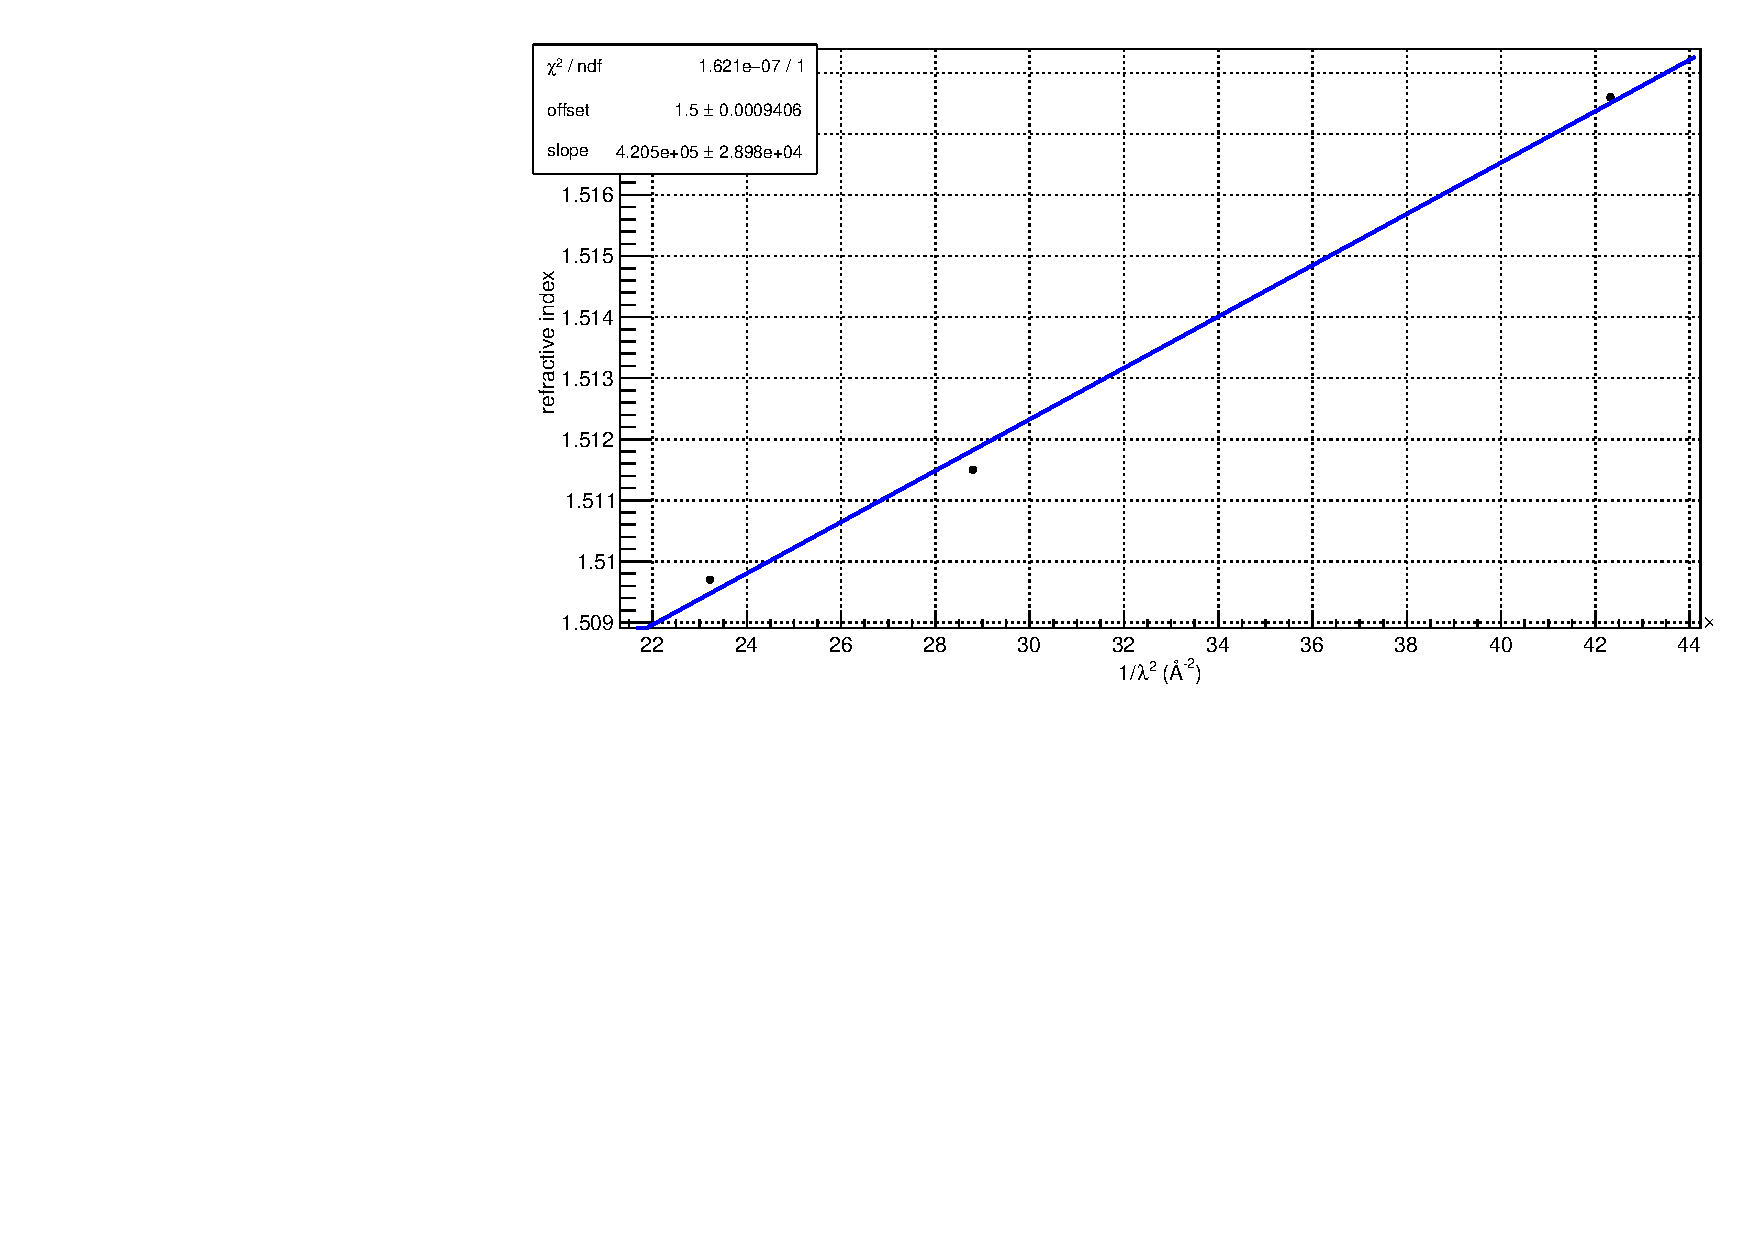
\includegraphics[scale=0.28, angle=0]{nFit}
%\caption{ Indice di rifrazione }
%\label{fig:alimentazione}
%\end{figure}
%\end{center}

	I parametri del fit sono :
	$$ A= 1.4997 \pm 0.0009 \quad B= (42 \pm 3 )10^4 \quad m^2$$
	Per $\lambda= 585.3 nm$ si ottiene quindi :
	$$n(\lambda)= 1.512 \pm 0.001  $$
	$$  \frac{dn}{d\lambda} = (-4.19 \pm 0.03 )\cdot 10^{-5} $$

	\section*{Aquisizione dati}
	
	\paragraph{Calibrazione}
	Prima di procedere con la presa dati si è eseguita una calibrazione 
	dell'apparato; in particolare occorre regolare la posizione 
	della sorgente rispetto all'apertura della fenditura.
	Il primo passaggio è stato quindi impostare l'apertura della fenditura 
	a $24 \mu m$ ed aquisire un primo spettro a lamina disinserita, con il 
	CCD orizzontale. Zoomando sui primi 3/4 picchi dello spettro, saremo
	in grado di individuare il nostro picco di interesse.
	Successivamente si è regolata ulteriormente la posizione della sorgente 
	cercando quella che massimizzi l'intensità e la forma del picco di 
	interesse.
	Si è quindi fissata la posizione del CCD a 0.93 mm e impostato l'apertura 
	della fenditura a $18 \mu m$.
	Infine si sono regolate le posizioni della lente focale e della lente 
	condensante, scegliendo come posizioni ottimali rispettivamente 15.36 mm 
	e 14.62 mm.


	\subsection*{Campo magnetico spento}

	Dopo la calibrazione si è proseguito con l'acquisizione del primo 
	spettro a campo magnetico spento: dopo aver selezionato il picco di 
	interesse si è inserito la lamina di Lummer-Gerhcker, e, selezionato 
	con i cursori il range dello scanning, si è ruotata il CCD
	in posizione verticale.
	Infine si è impostato un tempo di integrazione di 600 ms e si è avviato
	lo scanning, dopo aver salvato il file nell'opportuna cartella.


	\paragraph{Analisi dello spettro}
	Per procedere con l'analisi dello spettro, si è caricata ed eseguita su root la macro ReadZeemanImage.C++. 
	Si è ottenuto quindi un istogramma bidimensionale, al quale si è sottratto il segnale di fondo riferendosi alla sua proiezione sull’asse x.
	Dopo aver sottratto il fondo, migliorando la nitidezza dell'immagine, si sono registrati i limiti della zona del segnale. 
	In questo modo si è quindi ottenuta anche la proiezione di tale regione sull’asse y, in cui si osservano una serie di picchi, 
	di cui si può migliorare la pulizia dell'immagine mediante un rebin.



	\paragraph{Analisi dei picchi}


	Per fornire un'analisi estesa dello spettro si è scelto di raggruppare
	i picchi in 6 terne di picchi consecutivi, e per ciascuna terna
	l'obiettivo è studiare le spaziature tra i picchi e caratterizzarne in
	qualche modo la larghezza. 
	In particolare si è scelto di eseguire un fit gaussiano sui picchi
	per poter individuare con precisione l'ordinata di massimo e per
	poter dare una stima della larghezza del picco come FWHM.

	Per prima cosa, studiamo l'andamento delle spaziature tra i picchi. 
	Per ciascuna terna, si sono calcolate le due distanze tra i valori medi
	delle tre gaussiane, considerandone poi la media aritmetica $\Delta x_{ru}$,
	disponendo così di un valore univoco per caiscuna terna.
	In particolare ci si aspetta per queste distanze un andamento quadratico 
	in funzione della posizione del CCD. Si è effettuata dunque un'interpolazione
	parabolica, con il fine di stimarne poi l'ordinata di vertice che 
	costituirebbe la distanza minima efficace da usare per la stima
	corretta dell'angolo di incidenza i. Tale stima corretta di i
	permette di calcolare $\Delta\lambda_{ru}$ evitando l'approssimnazione $i \approx \pi$/2. 
	Maggiori dettagli sono riportati alla fine di questa sezione.
	Avendo a disposizione il valore medio della spaziatura tra i picchi per ciascuna
	terna, si è calcolato il fattore di calibrazione valido per quella regione
	di spettro, secondo il rapporto

	\begin{equation}
		F = \frac{\Delta\lambda_{ru}}{\Delta x_{ru}}.
	\end{equation}

	Il fattore di calibrazione F rappresenta il fattore di conversione da pixel, 
	ossia l'unità di misura caratteristica del CCD, in metri.

	%CONTINUO QUI NESSUNO SI PERMETTA
s





	\paragraph{Stima dell'angolo di incidenza sulla lamina di Lummer-Gehrcker}
	Si è accennato in precedenza che i raggi di luce incidono quasi radenti
	alla lamina. In particolare è possibile efettuare una stima precisa dell'
	angolo di incidenza. Occorre innanzitutto calcolare l'apertura angolare
	$\Delta i$, calcolata dal rapporto $\Delta x_{ru}$/f, dove f = 0.25 m è la distanza
	focale della lente e il valore di $\Delta x_{ru}$ è ottenuto dall'ordinata 
	di vertice del fit parabolico. Successivamente si applica la relazione

	\begin{equation}
		\sin(2i) = - \frac{\lambda \sqrt{n^2-1}}{d \Delta i}
	\end{equation}

	da cui si è potuto ottenere una stima dell'angolo i, in particolare

	\[
		i = 1.568 pm 0.003 rad = ( 89.8 \pm 0.2 ) ^{°}
	\]

	Il valore è compatibile con l'approssimazione a 90°, e inserendolo in \ref{eqn:dlru}
	si otterrà la miglior stima del range di lunghezza d'onda efficace usata
	nel calcolo dei fattori di calibrazione.


	\section*{Conclusioni}



	\newpage
	\appendix
	\section{Appendici}
	\label{appendice}
	\subsection{Costruzione dell'errore sulle misure}
	\label{Calcerr}

	\subsection{Tabella delle compatibilità}
	\medskip
	\begin{table}[H]
		\centering
		\begin{tabular}{c}
			%\hline
			\begin{Large}
			$\lambda=\frac{|a-b|}{\sqrt{\sigma_a^2+\sigma_b^2}}$
			\end{Large}\\
			%\hline
		\end{tabular}
		\hspace{0.5cm}
		\begin{tabular}{cc}
			\toprule
			&       \textbf{Compatibilità   }       \\
			\midrule
			0$\leq \lambda$<1   &Ottima                 \\
			1$\leq \lambda$<2   &Buona                  \\
			2$\leq \lambda$<3   &Accettabile            \\
			3$\leq\lambda$<5   &Pessima                \\
			$ \lambda \geq $  5     &Non compatibile        \\
			\bottomrule
		\end{tabular}
		\caption{indicazioni lettura compatibilità}
		\label{tab:compatibilità}
	\end{table}

	\subsection{Dati sperimentali}


   
\end{document}
